\documentclass[a4paper,10pt,openright]{report}
\setlength{\parindent}{0pt} % set noindent for entire file

\usepackage[utf8]{inputenc}
\usepackage[a4paper,top=20mm,bottom=25mm,left=10mm,right=10mm]{geometry}
\usepackage{xcolor,graphicx}
\usepackage{amsmath}
\usepackage{setspace}
\usepackage{sectsty}
\usepackage{etoolbox}
\usepackage{enumitem}
\usepackage{listings}
\usepackage{textcmds}
\usepackage{times}

\graphicspath{ {/home/saran/Analytics/May_05/} }

\lstdefinestyle{mystyle}{
	backgroundcolor=\color{white},
	basicstyle=\ttfamily\footnotesize,
	breakatwhitespace=false,
	breaklines=true,
	captionpos=b,
	keepspaces=true,
	showspaces=false,
	showstringspaces=false,
	showtabs=false,
	tabsize=4
}

\lstset{style=mystyle}

\begin{document}
\singlespacing
\pagestyle{plain}

\begin{center}
\textbf{Assignment z-test} \\
Date: 05/05/2020 \hspace{2mm} Name: D.Saravanan
\end{center}

\vspace{10px}

\begin{enumerate}

\item[1.] A sample of 400 male students is found to have a mean height of 171.38 cm. Can it
be reasonably regarded as a sample from a large population with mean height 171.17 cm and
standard deviation 3.30 cm. \\

\textbf{Solution:}

Given that $n = 400$, $\bar x = 171.38$ cm, $\mu = 171.17$ cm, $\sigma = 3.30$ cm \\ 

Sample proportion:
\begin{equation*}
p = \frac{\bar x}{n} = \frac{171.38}{400} = 0.42845
\end{equation*}

\textbf{Null hypothesis:} $H_{0}: \mu = 171.17$ \\
\textbf{Alternative hypothesis:} $H_{1}: \mu \neq 171.17$ \hspace{5px} (two tailed test)

$z$-statistic:
\begin{equation*}
z = \frac{\bar x - \mu}{\sigma/\sqrt{n}}
  = \frac{171.38 - 171.17}{3.30/\sqrt{400}}
  = 1.27273
\end{equation*}

At $5\%$ significance level the tabulated value for $z_{\alpha}$ is $1.96$ 

\textbf{Conclusion:} $|z| < z_{\alpha}$, we accept the Null hypothesis. That is there is no
significant difference between the sample mean and the population mean. \\

$95\%$ fiducial limits (Confidence Interval): \\
The confidence interval for the population mean is given by 

\begin{equation*}
\begin{split}
&\bar x \pm z_{\alpha} \frac{\sigma}{\sqrt{n}} \\
&171.38 \pm 1.96 \frac{3.30}{\sqrt{400}} = 171.38 \pm 0.3234
\end{split}
\end{equation*}

Program:
\lstinputlisting[language=Python]{tscript.py}

Output:
\lstinputlisting{toutput1a.txt}

%figure_1
\begin{figure}[ht!]
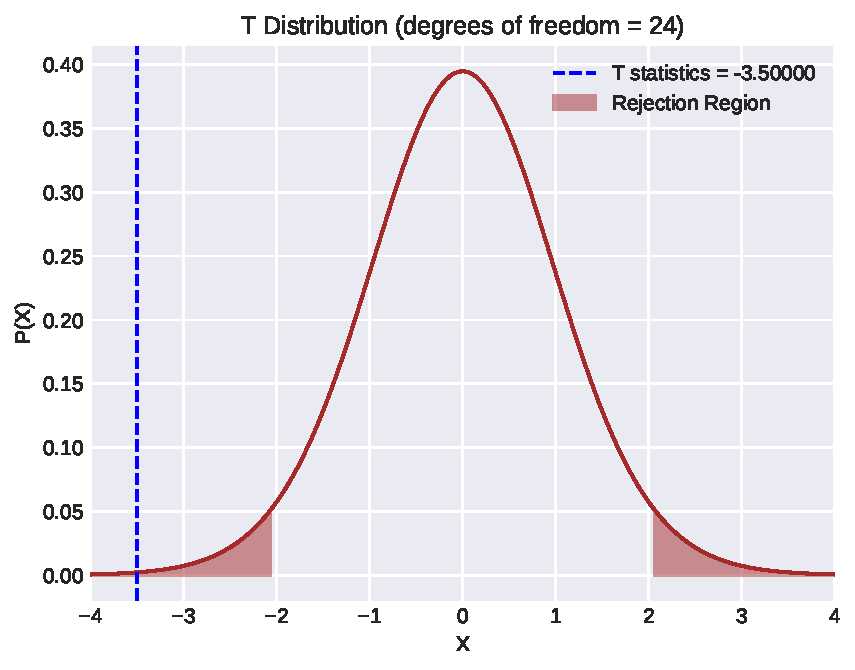
\includegraphics[width=14cm,height=7cm,keepaspectratio]{tscript1a.pdf}
\centering
\end{figure}

\item[2.] A sample of 900 items has mean 3.4 and standard deviation 2.61 Can the sample be
regarded as drawn from a population with mean 3.25 at 1 percent level of significane. \\

\textbf{Solution:}

\textbf{Null hypothesis:} $H_{0}: \mu = 3.25$ \\
\textbf{Alternative hypothesis:} $H_{1}: \mu \neq 3.25$ \hspace{5px} (two tailed test) \\

Program:
\lstinputlisting[language=Python]{tscript2.py}

\pagebreak

Output:
\lstinputlisting{toutput2.txt}

%figure_3
\begin{figure}[ht!]
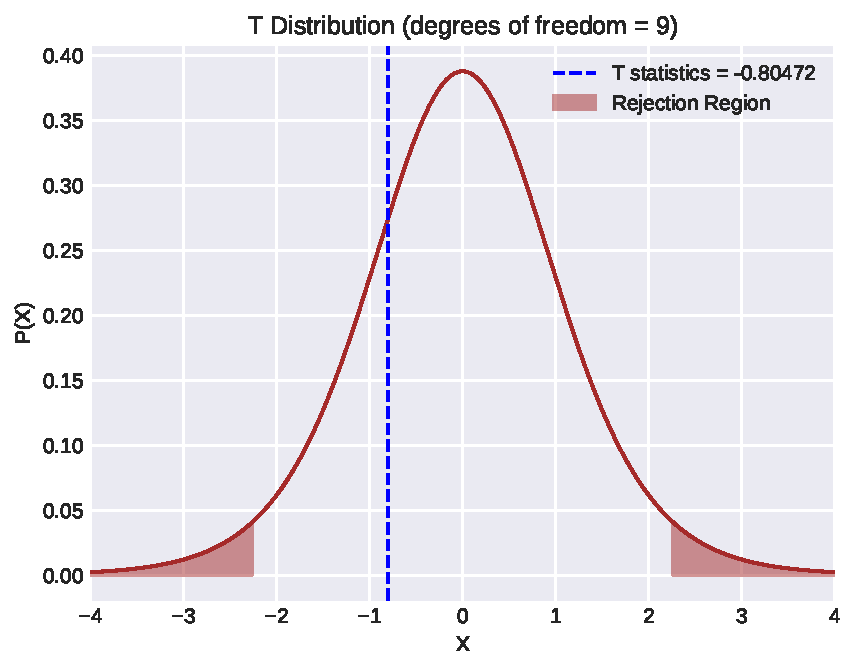
\includegraphics[width=14cm,height=7cm,keepaspectratio]{tscript2.pdf}
\centering
\end{figure}

\end{enumerate}
\end{document}
